\let\texyear\year
\documentclass{ieeeaccess}
\let\ieeeaccessyear\year
\let\year\texyear

\usepackage{cite}
\usepackage{amsmath,amssymb,amsfonts,amsthm,mathtools}
\usepackage{graphicx}
\usepackage{booktabs,array}
\usepackage{enumitem}
\usepackage{url}
\usepackage{tikz}
\urlstyle{tt}
\makeatletter
\g@addto@macro\UrlBreaks{\do\_\do\-}
\makeatother
\usetikzlibrary{arrows.meta,positioning,decorations.pathreplacing,automata,calc}
% Unified monochrome figure style for the paper.
% All automata and timing diagrams use white states, black borders and black arrows.
\tikzset{
  fmbracebottom/.style={
    decorate,
    decoration={brace,mirror,amplitude=4pt}
  },
  fmstate/.style={
    circle, draw=black, fill=white, line width=0.6pt,
    minimum size=9mm, inner sep=1pt, font=\small
  },
  fmstatewide/.style={
    rounded rectangle, draw=black, fill=white, line width=0.6pt,
    minimum height=8mm, inner xsep=3pt, inner ysep=1.5pt, font=\small
  },
  fmaccept/.style={fmstate,double,double distance=1.2pt},
  fmerror/.style={fmstate,double,double distance=1.2pt,fill=white},
  fmedge/.style={->,>=Stealth,line width=0.6pt},
  fmlabel/.style={font=\scriptsize,align=center,fill=white,inner sep=1.2pt},
  fminvariant/.style={font=\scriptsize,align=center},
  fmnote/.style={font=\scriptsize,align=center},
  fmtimeline/.style={->,>=Stealth,line width=0.6pt},
  fmevent/.style={circle,draw=black,fill=white,line width=0.6pt,minimum size=4.5mm,inner sep=0.5pt},
  fmreference/.style={fmevent,double,double distance=0.8pt},
  fmguide/.style={densely dashed,line width=0.45pt},
  fmbrace/.style={decorate,decoration={brace,amplitude=4pt},line width=0.5pt}
}

% The official class declares its blue as a Pantone spot color. Some PDF
% renderers cannot resolve the emitted spot-color resource, making the title
% and headings disappear. Override it after xcolor is loaded with the same
% declared CMYK alternate as a process color; class and layout stay intact.
\definecolor{accessblueprocess}{cmyk}{1,0.3,0,0.2}
\colorlet{accessblue}{accessblueprocess}

\newtheorem{theorem}{Theorem}[section]
\newtheorem{lemma}[theorem]{Lemma}
\newtheorem{corollary}[theorem]{Corollary}
\newtheorem{proposition}[theorem]{Proposition}
\newtheorem{assumption}[theorem]{Assumption}
\newtheorem{definition}[theorem]{Definition}

\newcommand{\Nat}{\mathbb{N}}
\newcommand{\Real}{\mathbb{R}}
\newcommand{\satM}{\models_{\mathrm{MTL}}}
\newcommand{\satL}{\models_{\mathrm{LTL}}}
\newcommand{\Until}{\mathbin{\mathsf{U}}}
\newcommand{\Release}{\mathbin{\mathsf{R}}}
\newcommand{\hUntil}{\mathbin{\widehat{\mathsf{U}}}}
\newcommand{\hRelease}{\mathbin{\widehat{\mathsf{R}}}}
\newcommand{\Next}{\mathsf{X}}
\newcommand{\Always}{\mathsf{G}}
\newcommand{\Eventually}{\mathsf{F}}
\newcommand{\WeakUntil}{\mathbin{\mathsf{W}}}
\newcommand{\Reset}{\mathsf{rst}}
\newcommand{\Unch}{\mathsf{unch}}
\newcommand{\T}{\mathcal{T}}
\newcommand{\Node}{\mathsf{node}}
\newcommand{\CVal}{\mathsf{val}}
\newcommand{\CReset}{\mathsf{reset}}
\newcommand{\elapsed}{\mathsf{elap}}
\newcommand{\ewbase}{\mathsf{ew\_base}}
\newcommand{\Clock}{\mathit{Clock}}
\newcommand{\runinhead}[1]{\par\noindent\textbf{#1}\enspace}
\newcommand{\Rocqid}[1]{\url{#1}}

\title{A Mechanically Verified Translation of MTL$_{0,\infty}$ into Timed B\"uchi Automata}

\author{\uppercase{Elie Fares}\authorrefmark{1},
\uppercase{Jean-Paul Bodeveix}\authorrefmark{2},
\uppercase{Hussain Al-Aqrabi}\authorrefmark{1} AND
\uppercase{Azar Salami}\authorrefmark{1}}
\address[1]{Higher Colleges of Technology, Sharjah, United Arab Emirates
 (e-mail: efares@hct.ac.ae, halaqrabi@hct.ac.ae, asalami@hct.ac.ae)}
\address[2]{IRIT, Universit\'e de Toulouse, France (e-mail: bodeveix@irit.fr)}
\corresp{Corresponding author: Elie Fares (e-mail: efares@hct.ac.ae).}
\markboth{Fares et al.: Mechanically Verified MTL-to-TBA Translation}
{Fares et al.: Mechanically Verified MTL-to-TBA Translation}

\begin{document}
\history{}
\doi{}

\begin{abstract}
Translation from real-time temporal specifications to timed automata supports
automated analysis, but depends on preserving the specified timed-word
language. We present a Rocq-checked soundness-and-completeness development for
the specified pointwise dense-time translation from Metric Temporal Logic
(MTL)$_{0,\infty}$ to timed B\"uchi automata (TBAs), via clocked Linear
Temporal Logic (LTL). Earlier work established mathematical language-preservation
results for this fragment; to the best of our knowledge, no published
machine-checked soundness-and-completeness development covers the particular
construction and semantic model formalized here. Rocq checks all eight strict
and non-strict primitive cases. The proof handles shared clocks and overlapping
activations by separating soundness for every clock-consistent reset trace
from completeness via one canonical reset trace and residual obligations. It
also checks relaxation and reset completion, yielding a compositional theorem
under an explicit all-words language-equivalence contract for the propositional
B\"uchi backend. For an alarm-response instance, we prove that a manually
transcribed backend record satisfies this contract and prove both an accepted
overlapping-alarm trace and a violating trace. The theorem uses real-valued
bounds, well-formed core formulas, strictly increasing divergent timestamps,
and event-guarded TBAs with existential initial clock valuations; the Spot
graph-to-record correspondence is outside the proof.
\end{abstract}

\begin{keywords}
Metric temporal logic, timed B\"uchi automata, Rocq, formal verification,
clocked LTL, semantic preservation.
\end{keywords}
\maketitle

\section{Introduction}
\label{sec:introduction}
Reliable translation from real-time Metric Temporal Logic (MTL) to timed
B\"uchi automata (TBAs) supports model checking and controller synthesis. Its
correctness is the semantic link between a temporal specification and the
automaton analyzed by a downstream tool. A bounded-response requirement, for example, is
\begin{equation*}
\Box(\mathit{req}\Rightarrow\Diamond_{\le d}\mathit{ack}).
\end{equation*}
Overlapping requests can leave several response obligations outstanding while
sharing the clock assigned to one primitive timed formula. Table~\ref{tab:overlap-example}
illustrates why the reset semantics need a correctness argument.

The mathematical construction studied here has substantial predecessors.
Bulychev et al. establish exact timed-automaton language results for safety
and co-safety fragments. Li et al. establish full-fragment
MTL$_{0,\infty}$-to-TBA language equality and show that their best-choice
reset policy preserves language~\cite{[BDLG14],li_spin7}. Their
work already contains the central timed-subformula clocking and reset
architecture. Our research result is a machine-checked proof for the specified
construction.

Mathematical proofs and machine-checked proofs provide different assurance.
A proof assistant requires the syntax, timed-word semantics, clock updates,
invariants, quantifiers, and proof dependencies to be represented in a
kernel-checkable development. Here that formalization must also reconcile
propositions of clocked Linear Temporal Logic (LTL) with genuine clock
valuations. Related proof-assistant
work addresses neighboring problems: Xu and Miao present a Metric Interval
Temporal Logic (MITL)-to-fair-timed-automaton construction and discuss its
implementation in the Prototype Verification System (PVS); Roohi and
Viswanathan mechanize results for MITL decision procedures in PVS; Schimpf et
al. verify an LTL-to-B\"uchi construction in Isabelle's higher-order logic
(HOL); Wang et al. verify a
Metric Linear Temporal Logic (MLTL)-to-regular-expression transformation in
Isabelle/HOL; and Chattopadhyay and Mamouras mechanize online monitoring for
past-time MTL under discrete-time quantitative semantics
\cite{xu08,roohi_viswanathan_vmcai18,schimpf_tphols09,
wang_mltl_tacas25,chattopadhyay_mamouras_rv20}. To the best of our knowledge,
no previous published machine-checked soundness-and-completeness development
has been identified for this particular pointwise MTL$_{0,\infty}$-to-TBA
construction and formal semantic model, including its clocked-LTL encoding,
relaxation, and reset-completion steps. This scoped claim recognizes the
existing proof-assistant work on related logics and constructions.

Several interacting proof obligations make the mechanization nontrivial.
Soundness must hold for every clock-consistent reset trace;
completeness must construct one trace that supports every dynamic activation
of a shared, formula-keyed clock. Independent witnesses per activation cannot
establish this single-trace property. The proof maintains residual obligations
for upper- and lower-bound Until and Release, and uses occurrence-indexed
structural induction so recursion through a syntax path retains the clock
identity of an identical primitive formula. Strict and non-strict boundaries
require distinct inequalities. In addition, the propositional backend can
assign clock atoms independently of actual clock valuations, so relaxation
and reset completion must preserve the precise implication directions before
the automaton theorem can be composed.

The principal contributions are:
\begin{itemize}
  \item Rocq-checked soundness and completeness of the clocked-LTL encoding,
        including all eight strict and non-strict hatted primitive cases and
        correctness at every syntactic occurrence;
  \item a canonical completeness construction that handles overlapping
        activations with one reset trace for each formula-keyed clock,
        together with policy-independent soundness for arbitrary consistent
        reset traces;
  \item checked relaxation and reset completion, composed with an explicit
        all-propositional-words backend contract in
        \Rocqid{MTL_to_TBA_correct_with}; and
  \item a concrete alarm-response instance whose manually transcribed Rocq
        backend satisfies the contract, with proved accepted-overlap and
        rejected-violation traces, and an inspectable proof and assumptions
        artifact.
\end{itemize}

The result is relative to the formal model defined here: real-valued bounds,
well-formed core formulas, strictly increasing divergent timestamps,
event-guarded TBAs without location invariants, and existential nonnegative
initial clocks. This differs from Li et al.'s integer-bound,
nondecreasing-time, zero-initial semantics and is not a direct refinement of
CASAAL's input/output semantics. The TBA theorem composes through an explicit
backend-equivalence premise; for the alarm instance Rocq checks a manually
transcribed backend record, not Spot or the graph-import path. Zero-bound
preprocessing is described but not verified, and the development proves a
semantic theorem rather than an executable compiler. Section~\ref{subsec:rocq-result-map}
summarizes the theorem dependencies and assumptions.
A related manuscript~\cite{fares_bodeveix_tba_optimization} addresses
downstream TBA optimization and UPPAAL-oriented export; that work and its
status are disclosed separately.

Section~\ref{sec:logic} defines the semantics and target model;
Sections~\ref{sec:translation}--\ref{sec:tba-construction} present the encoding and
automaton construction; Section~\ref{sec:correctness} develops the proof and
includes the alarm-response instance in Section~\ref{sec:alarm-example};
Section~\ref{sec:artifact} describes the artifact and reproduction procedure,
and Section~\ref{sec:related} discusses related work before the conclusion
.
\section{Logic and Semantic Model}
\label{sec:logic}
\subsection{Pointwise MTL$_{0,\infty}$}
\label{sec:mtl}
Let $\Sigma$ be a finite set of actions. Formulas are in negation normal
form and use Boolean operators, next, untimed Until and Release, and timed
Until and Release whose intervals have one endpoint at zero or infinity.
We write a bound as $\sim d$, with $\sim\in\{<,\le,>,\ge\}$. The logic also
contains the hatted operators $\hUntil_{\sim d}$ and
$\hRelease_{\sim d}$. In a hatted operator the current position is skipped
by the logical interval, while its timestamp remains the timing reference.
We use $\widehat{\Box}_{\sim d}\varphi$ as shorthand for
$\bot\hRelease_{\sim d}\varphi$; it requires $\varphi$ at each strictly
future position whose elapsed time from the current position satisfies the
bound.

A timed word is $w=(a_i,t_i)_{i\in\Nat}$, where $a_i\in\Sigma$,
$0\le t_0<t_1<\cdots$, and timestamps diverge. We write
$\elapsed_w(i,j)=t_j-t_i$. For Until, $w,i\satM p\Until_{\sim d}q$
holds when some $j\ge i$ satisfies $q$ and $t_j-t_i\sim d$, with $p$ at
each position in $[i,j)$. For hatted Until, the witness is $j>i$ and $p$
is required on $(i,j)$. Release is the dual universal condition: at every
position in the bounded region, either $q$ holds or $p$ held earlier in the
corresponding interval. Hatted Release excludes the current position from
that region. We use the standard pointwise semantics~\cite{MTLsem}.

For precision, the four bounded clauses used below are:
\begin{align*}
 w,i\satM p\Until_{\sim d}q
 &\Longleftrightarrow \exists j\ge i.\; w,j\satM q\\
 &\quad\land t_j-t_i\sim d\\[-1mm]
 &\quad\land \forall k\in[i,j).\;w,k\satM p,\\
 w,i\satM p\hUntil_{\sim d}q
 &\Longleftrightarrow \exists j>i.\; w,j\satM q\\
 &\quad\land t_j-t_i\sim d\\[-1mm]
 &\quad\land \forall k\in(i,j).\;w,k\satM p,\\
 w,i\satM p\Release_{\sim d}q
 &\Longleftrightarrow \forall j\ge i.\\[-1mm]
 &\quad\Bigl(t_j-t_i\sim d\Rightarrow\\[-1mm]
 &\qquad\Bigl(w,j\satM q\\[-1mm]
 &\qquad\quad\lor \exists k\in[i,j).\;w,k\satM p\Bigr)\Bigr),\\
 w,i\satM p\hRelease_{\sim d}q
 &\Longleftrightarrow \forall j>i.\\[-1mm]
 &\quad\Bigl(t_j-t_i\sim d\Rightarrow\\[-1mm]
 &\qquad\Bigl(w,j\satM q\\[-1mm]
 &\qquad\quad\lor \exists k\in(i,j).\;w,k\satM p\Bigr)\Bigr).
\end{align*}
The index intervals select event positions, whereas $t_j-t_i$ measures
elapsed physical time. Thus, when a bound falls between two events, no event
occurs exactly at that bound, and interval membership is still evaluated at
the event positions.
The strict increase assumption excludes simultaneous events; divergence is
used in the lower-bounded Until fairness argument.

The Rocq development represents action names by natural numbers rather than a
parameterized finite type, and timed words may use any natural-number name.
Each formula mentions finitely many names, so its semantics and generated
labels distinguish actions only by equality or inequality with those names.
Equivalently, the construction operates over the finite quotient induced by
those action tests; this is the finite alphabet used in the mathematical
presentation.

The well-formedness condition requires $d>0$ for every lower bound and strict
upper bound, and $d\ge0$ for a non-strict upper bound. Ordinary timed
operators are definitions in the mechanized core. For upper bounds
$\precsim\in\{\le,<\}$ and lower bounds $\succsim\in\{\ge,>\},$ they are:
\begin{align}
p\Until_{\precsim d}q &\equiv q\lor(p\land(p\hUntil_{\precsim d}q)),\label{eq:derive-ule}\\
p\Until_{\succsim d}q &\equiv p\land(p\hUntil_{\succsim d}q),\label{eq:derive-uge}\\
p\Release_{\precsim d}q &\equiv q\land(p\lor(p\hRelease_{\precsim d}q)),\label{eq:derive-rle}\\
p\Release_{\succsim d}q &\equiv p\lor(p\hRelease_{\succsim d}q).\label{eq:derive-rge}
\end{align}
These definitions separate the current-position case from the strictly future
obligation. Their pointwise semantic compatibility, including the stated
bound hypotheses, is proved in Rocq:
\begin{theorem}[Semantic compatibility of the derived timed operators]
\label{thm:derived-semantic-compatibility}
Under the well-formedness conditions above, Eqs.~\eqref{eq:derive-ule}--
\eqref{eq:derive-rge} agree with the standard pointwise semantics for all
strict and non-strict upper and lower bounds.
\end{theorem}
The identities follow by separating the current-position case from a
strictly future endpoint. For upper Until, a witness at $i$ contributes
$q$; every later witness requires $p$ at $i$ and leaves the hatted
obligation. A lower bound with $d>0$ excludes $i$, so $p$ is required now
and the remaining witness is hatted. The Release identities are the dual
case split: an upper-bound region includes $i$ and therefore requires $q$
there, while a lower-bound region excludes $i$. Strict upper bounds also
require $d>0$, avoiding the degenerate $<0$ case. The eight corresponding
Rocq lemmas are mapped to their source modules and assumptions in
Table~\ref{tab:rocq-result-map}.
Thus only
the eight hatted timed constructors require primitive translation clauses.
If a source formula has a zero lower bound, strict increase of timestamps
makes every strictly future elapsed time positive. At the hatted level,
$\hUntil_{\ge0}$ and $\hUntil_{>0}$ therefore reduce to
$\Next(p\Until q)$, while $\hRelease_{\ge0}$ and $\hRelease_{>0}$
reduce to $\Next(p\Release q)$. For ordinary operators, the current-position
case must also be simplified: the $\ge0$ cases are the corresponding untimed
Until and Release operators, and the $>0$ cases reduce to
$p\land\Next(p\Until q)$ and $p\lor\Next(p\Release q)$,
respectively. These reductions rely on the paper's strictly increasing event
times and must be applied before encoding a source formula as a Rocq core
formula; the preprocessing itself is not mechanized. A zero strict
upper bound has an empty interval: Until reduces to $\bot$ and Release to
$\top$; strict upper-bound constructors in the core consequently require
$d>0$. For the non-strict upper bound zero, the hatted future operators reduce
to $\hUntil_{\le0}\equiv\bot$ and $\hRelease_{\le0}\equiv\top$, because all
strictly future events have positive elapsed time. The derived ordinary
operators therefore both reduce to their right operand:
$p\Until_{\le0}q\equiv q$ and $p\Release_{\le0}q\equiv q$. These reductions
make the boundary explicit: the mechanized domain excludes zero lower bounds
and zero strict upper bounds, but includes non-strict upper bound zero.

\begin{figure}[t]
\centering
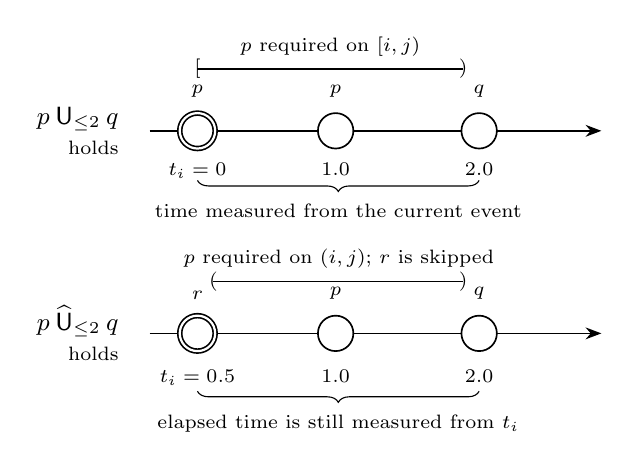
\begin{tikzpicture}[x=1.35cm,y=1.05cm,
  ival/.style={line width=0.5pt},
  ivallab/.style={font=\scriptsize,above=1pt}]
  % Ordinary Until
  \node[anchor=east,font=\small,align=right] at (-0.20,1.30) {$p\Until_{\le 2}q$\\{\scriptsize holds}};
  \draw[fmtimeline] (0,1.30) -- (4.25,1.30);
  \node[fmreference] (u0) at (0.45,1.30) {};
  \node[fmevent] (u1) at (1.75,1.30) {};
  \node[fmevent] (u2) at (3.10,1.30) {};
  \node[above=2pt of u0,font=\scriptsize] {$p$};
  \node[above=2pt of u1,font=\scriptsize] {$p$};
  \node[above=2pt of u2,font=\scriptsize] {$q$};
  \node[below=1.5pt of u0,font=\scriptsize] {$t_i=0$};
  \node[below=1.5pt of u1,font=\scriptsize] {$1.0$};
  \node[below=1.5pt of u2,font=\scriptsize] {$2.0$};
  \draw[ival] (0.45,2.05) -- (2.95,2.05);
  \node[font=\scriptsize] at (0.45,2.05) {$[$};
  \node[font=\scriptsize] at (2.95,2.05) {$)$};
  \node[ivallab] at (1.70,2.05) {$p$ required on $[i,j)$};
  \draw[fmbracebottom] (0.45,0.70) -- node[below=5pt,font=\scriptsize] {time measured from the current event} (3.10,0.70);

  % Hatted Until
  \node[anchor=east,font=\small,align=right] at (-0.20,-1.15) {$p\hUntil_{\le 2}q$\\{\scriptsize holds}};
  \draw[fmtimeline] (0,-1.15) -- (4.25,-1.15);
  \node[fmreference] (h0) at (0.45,-1.15) {};
  \node[fmevent] (h1) at (1.75,-1.15) {};
  \node[fmevent] (h2) at (3.10,-1.15) {};
  \node[above=2pt of h0,font=\scriptsize] {$r$};
  \node[above=2pt of h1,font=\scriptsize] {$p$};
  \node[above=2pt of h2,font=\scriptsize] {$q$};
  \node[below=3pt of h0,font=\scriptsize] {$t_i=0.5$};
  \node[below=3pt of h1,font=\scriptsize] {$1.0$};
  \node[below=3pt of h2,font=\scriptsize] {$2.0$};
  \draw[ival] (0.60,-0.52) -- (2.95,-0.52);
  \node[font=\scriptsize] at (0.60,-0.52) {$($};
  \node[font=\scriptsize] at (2.95,-0.52) {$)$};
  \node[ivallab] at (1.78,-0.52) {$p$ required on $(i,j)$; $r$ is skipped};
  \draw[fmbracebottom] (0.45,-1.85) -- node[below=5pt,font=\scriptsize] {elapsed time is still measured from $t_i$} (3.10,-1.85);
\end{tikzpicture}

\caption{Ordinary and hatted Until. The double circle is the timing reference.
The hatted operator skips the current event logically but measures from its
timestamp.}
\label{fig:hatted-until}
\end{figure}

This distinction is useful for sporadicity: if consecutive occurrences of
$e$ must be separated by at least $\theta$, one may write
$\Box(e\Rightarrow\widehat{\Box}_{<\theta}\neg e)$. The hatted form retains
the triggering event as the time origin; ordinary bounded temporal
operators do not express this particular reference shift directly.
Related pointwise MTL constructions and the CASAAL translation are discussed
in prior work~\cite{ouaknine_worrell_lics05,bouyer_chevalier_markey_fsttcs05,li_spin7,casaal_tool}.

\subsection{Timed B\"uchi Automata}
\label{sec:tba}
The verified target is an event-guarded TBA
$\mathcal A=(L,\ell_0,X,E,\mathit{Acc})$. Here $L$ is a finite set of
locations, $\ell_0$ the initial location, $X$ a finite set of clocks,
$E\subseteq L\times\mathsf{Lab}\times\mathsf{Guard}\times 2^X\times L$
is the set of action-labelled transitions with guards and reset sets, and
$\mathit{Acc}\subseteq L$ the B\"uchi set. A run is a sequence
$(\ell_i,v_i)_{i\ge0}$ starting at $\ell_0$; it follows one transition per
event and visits $\mathit{Acc}$ infinitely often. If the selected edge at
event $i$ is $(\ell_i,\alpha_i,g_i,Z_i,\ell_{i+1})$, then the event action
must satisfy $\alpha_i$ and the valuation $v_i$ must satisfy every guard in
$g_i$. There are no location invariants in this model: timing constraints
are checked at the events of the timed word. This is the TBA record
represented in Rocq; the theorem does not cover a richer invariant-bearing
automaton model without an additional encoding.

Let $v_i$ be the clock valuation tested at event $i$ and
$\Delta_i=t_{i+1}-t_i$. A transition at event $i$ tests $v_i$ before its
reset decision; the next valuation is
\[
v_{i+1}(x)=
\begin{cases}
\Delta_i,&x\in Z_i,\\
v_i(x)+\Delta_i,&\text{otherwise.}
\end{cases}
\]
The initial nonnegative valuation $v_0$ is existentially quantified, as in
the Rocq clock-consistent-extension semantics; standard zero initialization
is not assumed.

\section{Clocked-LTL Translation}
\label{sec:translation}
\subsection{Shared clock identities}
The translation is structural. It maps Boolean and untimed temporal
operators homomorphically and maps each primitive timed subformula to an LTL
formula over an extended alphabet. For each action $a$, the extended
alphabet contains distinct action atoms $\mathsf{LAct}(a)$ and
$\mathsf{LNAct}(a)$, as well as clock-related atoms: clock comparisons
$x\sim d$, a reset atom
$\Reset(x)$, and a preservation atom $\Unch(x)$. Under timed-word
interpretation, the action atoms mean that the current action is $a$ or is
different from $a$, respectively. The atom $\mathsf{LNAct}(a)$ and the
negated literal of $\mathsf{LAct}(a)$ have the same timed-word interpretation,
but remain distinct propositions to the unconstrained LTL backend. The reset
and preservation atoms describe the clock update at the current event. Clock
values are read before the event's reset, matching the guard semantics of a
timed automaton.

For formula $f$, let $\Clock(f)$ be its finite set of distinct primitive
hatted timed subformulas. The clock associated with $F\in\Clock(f)$ is
$x=F$ itself. Clock identity uses structural equality on the Rocq MTL syntax
tree, with bounds compared by equality in $\Real$. Constructor, operands,
comparison, and bound all participate: identical formula values at different
paths share a clock, while semantic equivalence alone does not. No
simplification-based merging is used. The main result proves that this clock
also serves all dynamic activations of its subformula.
The clock count is therefore bounded by the number of distinct primitive
timed subformulas, which is at most the number of timed occurrences in $f$.
If structural subformulas are represented as shared nodes, the translation
can share their LTL encodings as well; this does not remove the usual
worst-case growth of an LTL-to-B\"uchi construction.

This clock-sharing policy is distinct from automaton-state minimization. The
reset trace is chosen for each formula identity as a whole. In particular,
the proof cannot justify the clock bound
by assigning a fresh clock to each activation and subsequently identifying
those clocks: it establishes directly that a single trace of reset decisions
for the formula is sufficient.

\subsection{Eight primitive clauses}
\label{sec:mtlbuchi}
Let $F$ be a primitive hatted formula at path $\pi$, with operands $p,q$.
Write $x=\mathsf{clock\_of}(F)$, $P=\T_{\pi0}(p)$,
$Q=\T_{\pi1}(q)$, and define
$\alpha\WeakUntil\beta=(\alpha\Until\beta)\lor\Always\alpha$.
For upper comparisons $\precsim\in\{\le,<\}$ and lower comparisons
$\succsim\in\{\ge,>\}$, complements are
$\le^{\mathrm c}=>$, $<^{\mathrm c}=\ge$, $\ge^{\mathrm c}=<$, and
$>^{\mathrm c}=\le$. The four clause shapes, each instantiated for its
strict and non-strict bound, give all eight primitive cases:
\begin{align}
\T_\pi(p\hUntil_{\precsim d}q)
 &=\Next\bigl(((x\precsim d)\land\Unch(x)\land P)\nonumber\\
 &\hspace{23mm}\Until((x\precsim d)\land Q)\bigr),\label{eq:t-hule}\\
\T_\pi(p\hUntil_{\succsim d}q)
 &=\Reset(x)\land\Next\bigl((P\Until((x\succsim d)\land(P\Until Q)))\nonumber\\
 &\hspace{23mm}\lor(\Always P\land\Always\Eventually Q)\bigr),\label{eq:t-huge}\\
\T_\pi(p\hRelease_{\precsim d}q)
 &=\Reset(x)\land\Next\bigl(Q\nonumber\\
 &\hspace{23mm}\WeakUntil((x\mathrel{\precsim^{\mathrm c}}d)\lor(P\land Q))\bigr),\label{eq:t-hrle}\\
\T_\pi(p\hRelease_{\succsim d}q)
 &=\Next\bigl(((x\mathrel{\succsim^{\mathrm c}}d)\land\Unch(x))\nonumber\\
 &\hspace{23mm}\WeakUntil((P\Release Q)\nonumber\\
 &\hspace{23mm}\lor((x\mathrel{\succsim^{\mathrm c}}d)\land P))\bigr).
 \label{eq:t-hrge}
\end{align}
The outer $\Next$ implements the hatted shift; $\Reset(x)$ and $\Unch(x)$
encode the restart and preservation choices. Until uses strong Until for a
bounded witness and weak Until for the Release window. Lower-bounded Until
also has a fairness branch for an obligation whose threshold is delayed
indefinitely. Every clock atom occurs positively, which is the property used
by relaxation in Section~\ref{sec:reset-completion}. The eight local proof
arguments establish the precise strict and non-strict behavior in
Section~\ref{subsec:primitive-soundness}.

\begin{table}[t]
\centering
\caption{Clock comparisons used by each hatted primitive.}
\label{tab:clock-tests}
\begin{tabular}{@{}lll@{}}
\toprule
Primitive role & Non-strict bound & Strict bound\\
\midrule
$\hUntil_{\precsim d}$ endpoint & $x\le d$ & $x<d$\\
$\hUntil_{\succsim d}$ threshold & $x\ge d$ & $x>d$\\
$\hRelease_{\precsim d}$ window end & $x>d$ & $x\ge d$\\
$\hRelease_{\succsim d}$ pre-threshold & $x<d$ & $x\le d$\\
\bottomrule
\end{tabular}
\end{table}

\subsection{Shared clocks under overlapping activations}
\label{subsec:overlap-motivation}
Hatted operators preserve the triggering timestamp while moving logical
evaluation to the next event. For example,
$\Box(e\Rightarrow\widehat{\Box}_{<\theta}\neg e)$ measures an exclusion
window from the triggering event. The leading next in an ordinary operator
would shift that reference, while omitting it also constrains the triggering
event. Figure~\ref{fig:hat-reference} contrasts these readings.
\begin{figure*}[t]
\centering
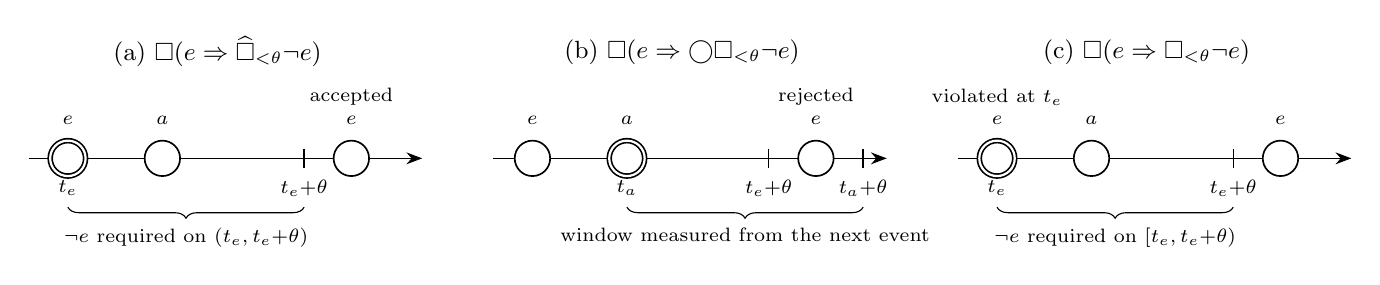
\begin{tikzpicture}[x=1cm,y=1cm,
  tick/.style={line width=0.5pt},
  ticklab/.style={font=\scriptsize,below=1pt},
  verdict/.style={fmnote}]
  % (a) Hatted operator: the intended reading
  \begin{scope}[xshift=0cm]
    \node[font=\small] at (2.4,1.35) {(a) $\Box(e\Rightarrow\widehat{\Box}_{<\theta}\neg e)$};
    \draw[fmtimeline] (0,0) -- (5.0,0);
    \node[fmreference] (a0) at (0.5,0) {};
    \node[fmevent] (a1) at (1.7,0) {};
    \node[fmevent] (a2) at (4.1,0) {};
    \node[above=2pt of a0,font=\scriptsize] {$e$};
    \node[above=2pt of a1,font=\scriptsize] {$a$};
    \node[above=2pt of a2,font=\scriptsize] {$e$};
    \node[verdict] at (4.1,0.78) {accepted};
    \draw[tick] (3.5,0.12) -- (3.5,-0.12) node[ticklab] {$t_e{+}\theta$};
    \node[ticklab] at (0.5,-0.12) {$t_e$};
    \draw[fmbracebottom] (0.5,-0.62) -- node[below=4pt,fmnote] {$\neg e$ required on $(t_e,t_e{+}\theta)$} (3.5,-0.62);
  \end{scope}

  % (b) Replacing the hat by a leading Next
  \begin{scope}[xshift=5.9cm]
    \node[font=\small] at (2.4,1.35) {(b) $\Box(e\Rightarrow\bigcirc\Box_{<\theta}\neg e)$};
    \draw[fmtimeline] (0,0) -- (5.0,0);
    \node[fmevent] (b0) at (0.5,0) {};
    \node[fmreference] (b1) at (1.7,0) {};
    \node[fmevent] (b2) at (4.1,0) {};
    \node[above=2pt of b0,font=\scriptsize] {$e$};
    \node[above=2pt of b1,font=\scriptsize] {$a$};
    \node[above=2pt of b2,font=\scriptsize] {$e$};
    \node[verdict] at (4.1,0.78) {rejected};
    \draw[tick] (3.5,0.12) -- (3.5,-0.12) node[ticklab] {$t_e{+}\theta$};
    \draw[tick] (4.7,0.12) -- (4.7,-0.12) node[ticklab] {$t_a{+}\theta$};
    \node[ticklab] at (1.7,-0.12) {$t_a$};
    \draw[fmbracebottom] (1.7,-0.62) -- node[below=4pt,fmnote] {window measured from the next event} (4.7,-0.62);
  \end{scope}

  % (c) Dropping the Next
  \begin{scope}[xshift=11.8cm]
    \node[font=\small] at (2.4,1.35) {(c) $\Box(e\Rightarrow\Box_{<\theta}\neg e)$};
    \draw[fmtimeline] (0,0) -- (5.0,0);
    \node[fmreference] (c0) at (0.5,0) {};
    \node[fmevent] (c1) at (1.7,0) {};
    \node[fmevent] (c2) at (4.1,0) {};
    \node[above=2pt of c0,font=\scriptsize] {$e$};
    \node[above=2pt of c1,font=\scriptsize] {$a$};
    \node[above=2pt of c2,font=\scriptsize] {$e$};
    \node[verdict] at (0.5,0.78) {violated at $t_e$};
    \draw[tick] (3.5,0.12) -- (3.5,-0.12) node[ticklab] {$t_e{+}\theta$};
    \node[ticklab] at (0.5,-0.12) {$t_e$};
    \draw[fmbracebottom] (0.5,-0.62) -- node[below=4pt,fmnote] {$\neg e$ required on $[t_e,t_e{+}\theta)$} (3.5,-0.62);
  \end{scope}
\end{tikzpicture}

\caption{The hatted sporadicity property and two ordinary-operator
substitutions. A leading next shifts the timing reference to the following
event; omitting it includes the triggering event in the window.}
\label{fig:hat-reference}
\end{figure*}

The proof assigns one clock to each structurally distinct primitive timed
formula, even when that formula is activated repeatedly. The finite prefix in
Table~\ref{tab:overlap-example} illustrates why completeness must account for
all pending obligations: resetting a single clock at the later request can
make an expired earlier deadline appear to be met. The table illustrates a
generic reset risk and makes no claim about an error in prior tools.
\begin{table}[t]
\centering
\caption{A finite prefix illustrating overlapping response obligations.
The deadline is five time units; the acknowledgment at time six is late for
the request at time zero even though it is age two from the later request.}
\label{tab:overlap-example}
\begin{tabular}{@{}clccc@{}}
\toprule
Event $i$ & Action & Time $t_i$ & Oldest age & Reset age\\
\midrule
0 & $\mathit{req}$ & 0 & 0 & 0\\
1 & $\mathit{req}$ & 4 & 4 & 4\\
2 & $\mathit{ack}$ & 6 & 6 & 2\\
\bottomrule
\end{tabular}
\end{table}
This is only motivation. The semantic proof below constructs one trace per
formula-keyed clock and establishes the residual invariants needed when
several activations are pending at once.

\section{From Clocked LTL to a TBA}
\label{sec:tba-construction}
\subsection{LTL-to-B\"uchi contract}
The backend treats extended atoms as independent propositions. It returns a
propositional B\"uchi automaton (PBA) whose language is exactly that of the
clocked-LTL formula. The theorem is stated for any such backend, deterministic
or not.
\begin{assumption}[Backend correctness]
\label{ass:backend}
For each formula $F$ and each propositional word $s$ over its atoms,
$\mathsf{PBA\_accepts}(A,s)$ iff $s,0\models F$, where $A$ is the backend
automaton for $F$.
\end{assumption}
This contract ranges over all propositional words, including assignments
that do not correspond to any clock-consistent timed word. That stronger
scope is used by relaxation.

\subsection{Relaxation and reset completion}
\label{sec:reset-completion}
The propositional backend regards every extended atom as independent. Its
correctness contract therefore applies to all Boolean words, including
assignments that cannot arise from any clock-consistent timed trace. Every
clock-related atom in the translation occurs positively. Relaxation acts on
each backend transition cube by removing negative literals over clock
comparisons and reset/preservation markers, removing irrelevant
clock-related literals, and discarding contradictory cubes. Action literals
and positive relevant clock literals are retained. This weakens the cubes
without asking the backend to understand clocks.

Reset completion converts each relaxed cube to a timed transition. A
preservation clock is reset unless the cube contains $\Unch(x)$; a restart
clock is reset exactly when the cube contains $\Reset(x)$. The markers are
then removed, clock comparisons become guards, and action literals become
labels. The two clock classes move in opposite directions, so the proof
treats them separately.

\begin{lemma}[Reset completion]
\label{lem:reset-completion}
Let an accepting run of the relaxed backend be accompanied by a
clock-consistent extension $\rho$ of its timed word. Reset completion
defines a clock-consistent extension $\rho'$ with the same timed word and
the same initial clock valuation. The same state sequence is an accepting
run of the completed TBA on $\rho'$.
\end{lemma}
\begin{proof}
Fix a selected backend cube at position $i$. For a preservation clock $x$,
if the cube contains $\Unch(x)$ then both traces preserve $x$. Otherwise the
completed TBA resets $x$, while $\rho$ may either reset it or preserve it.
Thus the completed reset set contains the original reset decision for $x$.
Induction on positions using the clock recurrence gives
$\CVal_{\rho'}(i,x)\le\CVal_\rho(i,x)$. These clocks occur only in upper
tests ($x\le d$ or $x<d$), which remain true when the value decreases.

For a restart clock $x$, completion resets it exactly when the cube contains
$\Reset(x)$. A true reset marker requires that $\rho$ resets $x$; without the
marker completion preserves it, whether or not $\rho$ resets it. The
completed reset set is therefore contained in the original one, and the same
induction gives $\CVal_{\rho'}(i,x)\ge\CVal_\rho(i,x)$. These clocks occur
only in lower tests ($x\ge d$, $x>d$, or their equivalent window-ending
comparisons), which remain true when the value increases. The clock recurrence
holds by the construction of $\rho'$. State transitions, event labels,
guards that remain true, and the Büchi accepting set are unchanged, so the
run remains accepting. Rocq proves this result as
\Rocqid{complete_complete}.
\end{proof}

The role of propositional valuations, relaxation, and reset completion in
both directions is proved once, as part of the end-to-end composition in
Theorem~\ref{thm:mtl-to-tba-correct}. A propositional model alone is not a
clock-consistent timed trace.
\subsection{Worked example: bounded eventuality with an exclusion window}
Let
\[
  f=(\Eventually_{\le5}p)\land(\Always_{<2}\neg p).
\]
It requires $p$ to be false at the origin and until age two, then true by age
five. Figure~\ref{fig:translation-reference-tba} shows a hand-simplified
equivalent one-clock TBA, not the syntax-directed output, which assigns
separate clocks to the two distinct timed subformulas. The steps below show
the clocked-LTL translation and timed reinterpretation. This is a construction
illustration: the saved Spot graph and its two-clock TBA transcription are not
covered by the proved Rocq backend contract. The mechanically verified
concrete instance is the alarm-response example in
Section~\ref{sec:alarm-example}.

\begin{figure}[t]
\centering
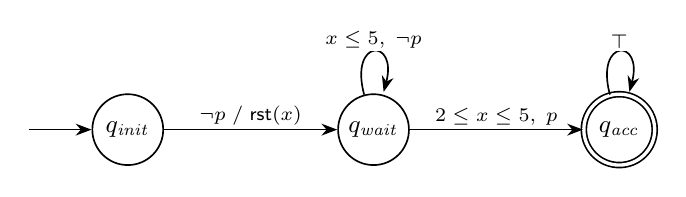
\begin{tikzpicture}[node distance=22mm]
  \node[fmstate] (q0) {$q_{\mathit{init}}$};
  \node[fmstate,right=of q0] (q1) {$q_{\mathit{wait}}$};
  \node[fmaccept,right=of q1] (q2) {$q_{\mathit{acc}}$};
  \draw[fmedge] ([xshift=-8mm]q0.west) -- (q0.west);
  \draw[fmedge] (q0) -- node[fmlabel,above] {$\neg p\;/\;\mathsf{rst}(x)$} (q1);
  \draw[fmedge] (q1) edge[loop above] node[fmlabel] {$x\le5,\;\neg p$} (q1);
  \draw[fmedge] (q1) -- node[fmlabel,above] {$2\le x\le5,\;p$} (q2);
  \draw[fmedge] (q2) edge[loop above] node[fmlabel] {$\top$} (q2);
\end{tikzpicture}

\caption{Hand-simplified equivalent event-guarded TBA for $f$. The initial
transition requires $\neg p$ and resets $x$; in the waiting location,
$x\le5$, and acceptance also requires $x\ge2$. Thus $p$ first holds at age
in $[2,5]$.}
\label{fig:translation-reference-tba}
\end{figure}

\begin{enumerate}[label=Step~\arabic*:,leftmargin=*]
\item The formula is in negation normal form. Expanding the derived operators
and applying the timed-operator identities gives
\[
\begin{aligned}
f
 &= (\top\Until_{\le5}p)\land(\bot\Release_{<2}\neg p)\\
 &= \bigl(p\lor(\top\land\top\hUntil_{\le5}p)\bigr)\\
 &\qquad\land\bigl(\neg p\land(\bot\lor\bot\hRelease_{<2}\neg p)\bigr).
\end{aligned}
\]
These current-position cases follow Eqs.~\eqref{eq:derive-ule} and
\eqref{eq:derive-rle}.

\item The two distinct primitive timed subformulas receive clocks $x$ and
$y$, respectively. Their clocked-LTL translation is
\begin{align*}
\Phi_U={}&p\lor\bigl(\top\land\Next\Bigl(
  ((x\le5)\land\Unch(x)\land\top)\Until\\[-1mm]
&\qquad((x\le5)\land p)\Bigr)\bigr),\\[-1mm]
\Phi_R={}&\neg p\land\bigl(\bot\lor(\Reset(y)\land\\[-1mm]
&\qquad\Next(\neg p\WeakUntil((y\ge2)\lor(\bot\land\neg p))))\bigr),\\[-1mm]
\T(f)={}&\Phi_U\land\Phi_R.
\end{align*}
The Until preserves $x$; the Release test $y\ge2$ complements the source
bound $<2$, allowing $p$ from age two.

\item The saved Spot 2.16 graph for $\T(f)$ is redrawn on the left of
Fig.~\ref{fig:translation-steps45}. Clock guards, reset and preservation
markers, and action atoms are independent propositions to the backend. In
particular, $p=\mathsf{LAct}(p)$ and $\neg p=\mathsf{LNAct}(p)$ are distinct
atoms, while $!p$ is the negated literal of $\mathsf{LAct}(p)$; a backend cube
may contain both $p$ and $\neg p$. Timed reinterpretation imposes action
consistency, so some backend edges have no realizable timed event.

\item Relaxation removes negative literals over extended clock atoms. Reset
completion resets the preservation clock $x$ unless $\Unch(x)$ is present;
the restart clock $y$ is reset exactly when $\Reset(y)$ is present. The right
side of Fig.~\ref{fig:translation-steps45} shows the same state graph after
these operations. Edge identifiers replace dense labels; Table~\ref{tab:worked-translation-edges}
gives each Spot cube and the corresponding event condition, surviving clock
guard, and completed reset set. The table retains unsatisfiable action cubes
to make the propositional-to-timed boundary visible; removing them would be a
subsequent simplification.
\end{enumerate}

\begin{figure*}[!t]
\centering
\resizebox{\textwidth}{!}{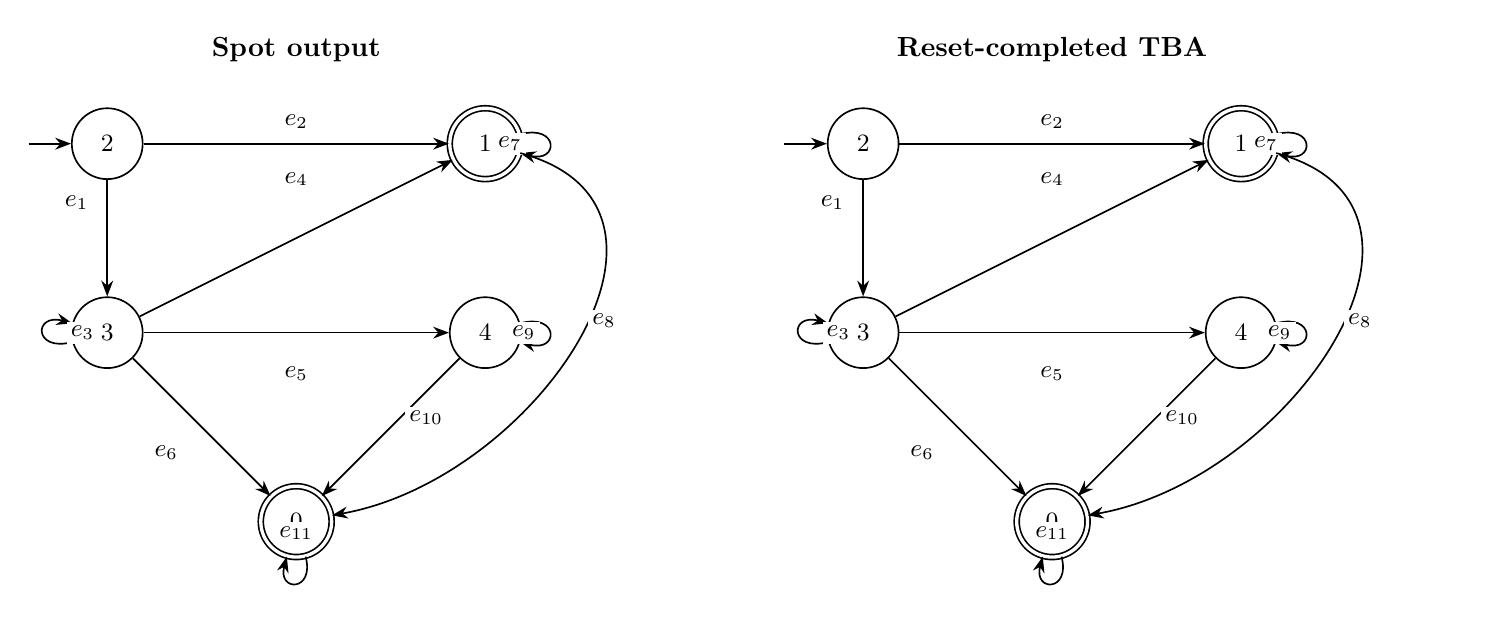
\begin{tikzpicture}[
  x=1cm,y=1cm,
  lab/.style={font=\small,align=center,fill=white,inner sep=1.5pt}
]
% Edge identifiers refer to Table~\ref{tab:worked-translation-edges}.
\begin{scope}[xshift=0cm]
  \node[fmnote,font=\normalsize\bfseries] at (2.4,6.0) {Spot output};
  \node[fmstate] (l0) at (0.0,4.8) {$2$};
  \node[fmstate] (l1) at (0.0,2.4) {$3$};
  \node[fmaccept] (l2) at (4.8,4.8) {$1$};
  \node[fmstate] (l3) at (4.8,2.4) {$4$};
  \node[fmaccept] (l4) at (2.4,0.0) {$0$};
  \draw[fmedge] (-1.0,4.8) -- (l0);
  \draw[fmedge] (l0) -- (l1);
  \node[lab,anchor=east] at (-0.18,4.05) {$e_1$};
  \draw[fmedge] (l0) -- (l2);
  \node[lab] at (2.4,5.08) {$e_2$};
  \draw[fmedge] (l1) edge[loop left,looseness=5.5] (l1);
  \node[lab,left,xshift=-3pt] at (l1) {$e_3$};
  \draw[fmedge] (l1) -- (l2);
  \node[lab] at (2.4,4.35) {$e_4$};
  \draw[fmedge] (l1) -- (l3);
  \node[lab] at (2.4,1.88) {$e_5$};
  \draw[fmedge] (l1) -- (l4);
  \node[lab] at (0.75,0.88) {$e_6$};
  \draw[fmedge] (l2) edge[loop right,looseness=5.5] (l2);
  \node[lab,right,xshift=3pt] at (l2) {$e_7$};
  \draw[fmedge] (l2) to[out=-15,in=10,looseness=1.3] (l4);
  \node[lab,right] at (6.1,2.55) {$e_8$};
  \draw[fmedge] (l3) edge[loop right,looseness=5.5] (l3);
  \node[lab,right,xshift=8pt] at (l3) {$e_9$};
  \draw[fmedge] (l3) -- (l4);
  \node[lab] at (4.05,1.32) {$e_{10}$};
  \draw[fmedge] (l4) edge[loop below,looseness=5] (l4);
  \node[lab,below] at (l4) {$e_{11}$};
\end{scope}

\begin{scope}[xshift=9.6cm]
  \node[fmnote,font=\normalsize\bfseries] at (2.4,6.0) {Reset-completed TBA};
  \node[fmstate] (r0) at (0.0,4.8) {$2$};
  \node[fmstate] (r1) at (0.0,2.4) {$3$};
  \node[fmaccept] (r2) at (4.8,4.8) {$1$};
  \node[fmstate] (r3) at (4.8,2.4) {$4$};
  \node[fmaccept] (r4) at (2.4,0.0) {$0$};
  \draw[fmedge] (-1.0,4.8) -- (r0);
  \draw[fmedge] (r0) -- (r1);
  \node[lab,anchor=east] at (-0.18,4.05) {$e_1$};
  \draw[fmedge] (r0) -- (r2);
  \node[lab] at (2.4,5.08) {$e_2$};
  \draw[fmedge] (r1) edge[loop left,looseness=5.5] (r1);
  \node[lab,left,xshift=-3pt] at (r1) {$e_3$};
  \draw[fmedge] (r1) -- (r2);
  \node[lab] at (2.4,4.35) {$e_4$};
  \draw[fmedge] (r1) -- (r3);
  \node[lab] at (2.4,1.88) {$e_5$};
  \draw[fmedge] (r1) -- (r4);
  \node[lab] at (0.75,0.88) {$e_6$};
  \draw[fmedge] (r2) edge[loop right,looseness=5.5] (r2);
  \node[lab,right,xshift=3pt] at (r2) {$e_7$};
  \draw[fmedge] (r2) to[out=-15,in=10,looseness=1.3] (r4);
  \node[lab,right] at (6.1,2.55) {$e_8$};
  \draw[fmedge] (r3) edge[loop right,looseness=5.5] (r3);
  \node[lab,right,xshift=8pt] at (r3) {$e_9$};
  \draw[fmedge] (r3) -- (r4);
  \node[lab] at (4.05,1.32) {$e_{10}$};
  \draw[fmedge] (r4) edge[loop below,looseness=5] (r4);
  \node[lab,below] at (r4) {$e_{11}$};
\end{scope}
\end{tikzpicture}
}
\caption{The saved Spot 2.16 graph (redrawn, left) and its hand-derived
reset-completed TBA (right; same state IDs). Edge identifiers are expanded in
Table~\ref{tab:worked-translation-edges}. This graph-to-TBA illustration is
not the formally verified alarm-response backend instance.}
\label{fig:translation-steps45}
\end{figure*}

\begin{table*}[!t]
\centering
\caption{Edge key for Fig.~\ref{fig:translation-steps45}. $P=\mathsf{LAct}(p)$,
$N=\mathsf{LNAct}(p)$, $n=\neg\mathsf{LAct}(p)$, $X=(x\le5)$,
$Y=(y\ge2)$, $U=\mathsf{LUnch}(x)$, and $R=\mathsf{LRst}(y)$. In the
timed interpretation, $P$ means event $p$ and both $N$ and $n$ mean event
$\neg p$. Negative $Y$ literals are removed by relaxation.}
\label{tab:worked-translation-edges}
\footnotesize
\begin{tabular}{@{}c c c p{0.37\textwidth} p{0.45\textwidth}@{}}
\toprule
Edge & From & To & Spot propositional cube & Timed event; guard; reset set\\
\midrule
$e_1$ & 2 & 3 & $N\land n\land R$ & $\neg p$; $\top$; $\{x,y\}$\\
$e_2$ & 2 & 1 & $N\land P\land R$ & $p\land\neg p$ (unrealizable); $\top$; $\{x,y\}$\\
$e_3$ & 3 & 3 & $N\land n\land U\land X\land\neg Y$ & $\neg p$; $x\le5$; $\varnothing$\\
$e_4$ & 3 & 1 & $N\land P\land X\land\neg Y$ & $p\land\neg p$ (unrealizable); $x\le5$; $\{x\}$\\
$e_5$ & 3 & 4 & $n\land U\land X\land Y$ & $\neg p$; $x\le5\land y\ge2$; $\varnothing$\\
$e_6$ & 3 & 0 & $P\land X\land Y$ & $p$; $x\le5\land y\ge2$; $\{x\}$\\
$e_7$ & 1 & 1 & $N\land\neg Y$ & $\neg p$; $\top$; $\{x\}$\\
$e_8$ & 1 & 0 & $Y$ & any event; $y\ge2$; $\{x\}$\\
$e_9$ & 4 & 4 & $n\land U\land X$ & $\neg p$; $x\le5$; $\varnothing$\\
$e_{10}$ & 4 & 0 & $P\land X$ & $p$; $x\le5$; $\{x\}$\\
$e_{11}$ & 0 & 0 & $\top$ & any event; $\top$; $\{x\}$\\
\bottomrule
\end{tabular}
\end{table*}

\cite{openai_codex}.

\section{Mechanized Correctness}
\label{sec:correctness}
\label{sec:encoding-correctness}
For a formula $f$, an extended word $\rho$ augments the timed word with a
nonnegative value $\CVal_\rho(i,x)$ and a reset decision
$\CReset_\rho(i,x)$ for every formula-keyed clock $x\in\Clock(f)$ at each
position $i$. It is clock-consistent when, with
$\Delta_i=t_{i+1}-t_i$,
\begin{equation}
\CVal_\rho(i+1,x)=
\begin{cases}
\Delta_i,&\CReset_\rho(i,x),\\
\CVal_\rho(i,x)+\Delta_i,&\text{otherwise.}
\end{cases}
\label{eq:clock-update}
\end{equation}
The value at $i$ is tested before the reset decision at $i$. The relation
$\mathsf{same\_base}(\rho,w)$ means that projection of $\rho$ onto actions
and timestamps gives $w$.

\subsection{Soundness for arbitrary reset traces}
\label{subsec:primitive-soundness}
The soundness direction does not select or assume the canonical policy. For
each primitive formula $F$ at path $\pi$, the corresponding Rocq lemma
\texttt{sound\_*} turns $\rho,i\models_{\mathrm{LTL}}\T_\pi(F)$ into
$\ewbase(\rho),i\models_{\mathrm{MTL}}F$, assuming clock consistency and
induction hypotheses for its operands. The four proof families below each
cover both the strict and non-strict comparison.

Clock consistency gives two useful bounds. If a clock is preserved on
$[i,j)$, then
\[
\CVal_\rho(j,x)=\CVal_\rho(i,x)+\elapsed_w(i,j).
\]
Since clock values are nonnegative, preservation implies
$\CVal_\rho(j,x)\ge\elapsed_w(i,j)$. If it is reset at $i$, then for every
$j\ge i+1$,
\[
\CVal_\rho(j,x)\le\elapsed_w(i,j),
\]
with equality when it is not reset again before $j$. The upper-guard
implication follows from the first inequality; the lower-guard implication
follows from the second. Both follow by induction from
Eq.~\eqref{eq:clock-update} and nonnegative delays.

\runinhead{Upper-bounded hatted Until.}
The outer $\Next$ moves to the first strictly future event. The strong Until
then supplies a witness $j>i$ satisfying $Q$, with $P$ at every intermediate
event and $\Unch(x)$ throughout that prefix. Regardless of whether the clock
was reset at $i$, its value at $i+1$ is at least $\Delta_i$.
Preservation after $i+1$ therefore gives
\[
\CVal_\rho(j,x)\ge
\Delta_i+\elapsed_w(i+1,j)=\elapsed_w(i,j).
\]
The endpoint guard $x\le d$ implies $\elapsed_w(i,j)\le d$; the guard $x<d$
implies $\elapsed_w(i,j)<d$. Induction on $P,Q$ yields the hatted Until
witness and prefix in both cases. The strong Until is essential: an infinite
continuation with no $Q$ endpoint is not a bounded Until witness.

\runinhead{Lower-bounded hatted Until.}
Here the translation requires $\Reset(x)$ at $i$. The finite branch of
$\Gamma$ waits for a position with $x\ge d$ (or $x>d$) and then supplies an
ordinary $P\Until Q$ witness. Since subsequent resets can only make a clock
younger, $\CVal_\rho(j,x)\le\elapsed_w(i,j)$; thus the threshold guard proves
the required lower-bound comparison. The nested Until supplies $P$ up to the
$Q$ witness. The other branch is
$\Always P\land\Always\Eventually Q$. It gives an unbroken $P$ prefix and
unboundedly many $Q$ positions; divergence of timestamps lets us choose a
$Q$ witness beyond any finite lower bound. For the strict case, choose a
recurring $Q$ at distance at least $d$ from $i+1$. Since
$t_{i+1}>t_i$, that same event is strictly more than $d$ after $i$. This is
the additional argument in \Rocqid{sound_UhatGt}; it preserves the strict
boundary without changing the constant.

\runinhead{Upper-bounded hatted Release.}
The translation resets the clock at $i$ and uses weak Until with $Q$ as its
left condition. Consequently, $Q$ holds at each future event until either
$P\land Q$ discharges the Release obligation or the complementary clock test
marks the end of the upper window. For a non-strict upper bound, the window
ends at $x>d$; for a strict upper bound, it ends at $x\ge d$. If the clock
has been reset again, its value is no larger than the elapsed time from $i$,
so either endpoint guard can hold only after the corresponding physical-time
window has ended. If weak Until ends at $P\land Q$, $P$ at that earlier event
discharges later Release obligations. This proves both comparisons with their
exact strict boundary.

\runinhead{Lower-bounded hatted Release.}
Before the threshold, the left side of weak Until requires both the
pre-threshold comparison and $\Unch(x)$. A non-strict lower bound uses
$x<d$; a strict lower bound uses $x\le d$. Thus an arbitrary reset trace
cannot move the clock backwards while the pre-threshold condition remains
active. Once the comparison becomes false, the translation requires ordinary
$P\Release Q$ from that event, unless the right-side alternative has already
terminated the obligation at a position satisfying $P$ while still below the
threshold. An older initial clock value can make the translation enter the
ordinary Release branch earlier than the MTL interval does; this only imposes
a stronger condition. The endpoint of the MTL lower interval is covered in
both cases, including the event exactly at $d$ for $\ge d$ and its exclusion
for $>d$.

The standard LTL semantics used here are formalized in Rocq as
\Rocqid{LG_semantics}, \Rocqid{LGF_semantics},
\Rocqid{LW_semantics}, and \Rocqid{LF_semantics}. Time divergence is used
only for the fairness witness in lower-bounded Until; no canonical-reset
assumption is used in any soundness family.

\subsection{Canonical reset policy and residual obligations}
\label{subsec:canonical-policy}
Completeness must choose one clock trace for each primitive formula, even
when activations overlap. The canonical policy preserves a reference only
while its residual obligation is still useful. Let
$\mathsf{elap}_w(i,j)=t_j-t_i$. For upper-bounded Until define
\begin{align}
\mathsf{URes}_{\le}(i,v,d,p,q)\iff{}\\[-1mm]
&\exists j\ge i.\;v+\elapsed_w(i,j)\le d\nonumber\\[-1mm]
&\land w,j\satM q\nonumber\\[-1mm]
&\land\forall k\in[i,j).\,w,k\satM p,\label{eq:ures-le}\\
\mathsf{URes}_{<}(i,v,d,p,q)\iff{}\\[-1mm]
&\exists j\ge i.\;v+\elapsed_w(i,j)<d\nonumber\\[-1mm]
&\land w,j\satM q\nonumber\\[-1mm]
&\land\forall k\in[i,j).\,w,k\satM p.\label{eq:ures-lt}
\end{align}
The residual says that a $q$ endpoint is still reachable with the current
clock age and the required $p$ prefix. For lower-bounded Release define
\begin{align}
\mathsf{RRes}_{\ge}(i,v,d,p,q)\iff{}\\[-1mm]
&\forall j\ge i.\;d\le v+\elapsed_w(i,j)\Rightarrow\nonumber\\[-1mm]
&\Bigl(w,j\satM q\lor\nonumber\\[-1mm]
&\exists k\in[i,j).\,w,k\satM p\Bigr),\label{eq:rres-ge}\\
\mathsf{RRes}_{>}(i,v,d,p,q)\iff{}\\[-1mm]
&\forall j\ge i.\;d<v+\elapsed_w(i,j)\Rightarrow\nonumber\\[-1mm]
&\Bigl(w,j\satM q\lor\nonumber\\[-1mm]
&\exists k\in[i,j).\,w,k\satM p\Bigr).\label{eq:rres-gt}
\end{align}
These are universal residuals: every position already beyond the threshold
must have $q$ or an earlier $p$ that discharges the obligation. Their
strict variants keep the comparison itself strict.

For a clock $x=F$, let $v=\CVal_{\rho^\star}(i,x)$. The policy is:
\begin{table}[t]
\centering
\caption{Canonical reset decision at position $i$. A preservation row gives
the condition under which the clock is not reset; otherwise it is reset.}
\label{tab:canonical-policy}
\begin{tabular}{@{}p{0.35\columnwidth}p{0.59\columnwidth}@{}}
\toprule
Primitive formula $F$ & Decision at $i$\\
\midrule
$p\hUntil_{\le d}q$ &
Preserve iff $v\le d$, $\mathsf{URes}_{\le}(i,v,d,p,q)$, and
$w,i\not\satM q$.\\
$p\hUntil_{<d}q$ &
Preserve iff $v<d$, $\mathsf{URes}_{<}(i,v,d,p,q)$, and
$w,i\not\satM q$.\\
$p\hUntil_{\ge d}q$, $p\hUntil_{>d}q$,
$p\hRelease_{\le d}q$, $p\hRelease_{<d}q$ &
Reset iff $w,i\satM F$.\\
$p\hRelease_{\ge d}q$ &
Preserve iff $v<d$, $\mathsf{RRes}_{\ge}(i,v,d,p,q)$, and
$w,i\not\satM p$.\\
$p\hRelease_{>d}q$ &
Preserve iff $v\le d$, $\mathsf{RRes}_{>}(i,v,d,p,q)$, and
$w,i\not\satM p$.\\
\bottomrule
\end{tabular}
\end{table}
The resulting values begin at $u_0=0$ and evolve by
\[
u_{i+1}=
\begin{cases}
\Delta_i,&\text{if the policy resets at }i,\\
u_i+\Delta_i,&\text{otherwise.}
\end{cases}
\]
This is a word-dependent completeness witness, not a reset algorithm in an
executable translator. Its decisions are keyed by the primitive formula
itself, not by an occurrence path.

\subsection{Completeness for one canonical trace}
\label{subsec:primitive-completeness}
For every satisfying formula, completeness constructs one clock-consistent
extension $\rho^\star$ that serves all activations of every shared clock.
The four operator families use different invariants; strict variants replace
each boundary test by its strict counterpart.

\runinhead{Upper-bounded hatted Until.}
Choose a future $q$ witness $j>i$ while the activation remains pending. The
key invariant along the translated strong-Until prefix is
\begin{equation}
\CVal_{\rho^\star}(n,x)+\elapsed_w(n,j)\le d
\quad(i<n\le j).
\label{eq:canonical-until-invariant}
\end{equation}
For $<d$, replace $\le d$ by $<d$. The invariant need not hold at $i$:
the translation begins with $\Next$, so the first clock test is at $i+1$.
If the policy resets at $i$, then $u_{i+1}=\Delta_i$ and
$u_{i+1}+\elapsed_w(i+1,j)=\elapsed_w(i,j)$, which is within the bound for
the chosen witness. If it preserves at $i$, the residual supplies a still
reachable $q$ endpoint and $p$ prefix; because the current $q$ has not
discharged that residual, its witness is strictly after $i$, and the same
identity advances the residual inequality to $i+1$. At every intermediate
event the policy either preserves this useful older reference or resets to a
new reference whose MTL obligation is true. The endpoint satisfies $q$ and
the clock comparison. An older reference is at least as old as a newer one,
so if it still reaches the shared endpoint within $d$, the shorter
newer-prefix obligations are covered as well. This is the invariant proved
by \Rocqid{complete_UhatLe} and \Rocqid{complete_UhatLt}.

\runinhead{Lower-bounded hatted Until.}
Whenever the formula is true at an activation, the policy resets its clock.
Starting from $i+1$, a first position at which the canonical clock reaches
$d$ (or strictly exceeds $d$) and has a qualifying later $q$ witness gives
the finite branch of $\Gamma$: the clock guard supplies the lower-bound
test, and the nested $P\Until Q$ supplies the remaining witness. Before the
first such position, the proof maintains an active-witness invariant. At
each $n\ge i+1$ it supplies an activation $s<n$, a witness $m\ge n$ with
$t_m-t_s\ge d$ and $w,m\models q$, $p$ at every intermediate position, and
$\CVal_{\rho^\star}(n,x)=t_n-t_s$. Thus $p$ holds at $n$ and a $q$ witness
remains at or after every $n$. If a first qualifying position occurs, the
finite branch applies; if none occurs, the invariant yields
$\Always P\land\Always\Eventually Q$, the fairness branch of $\Gamma$.
Divergence converts recurring $q$ positions into a witness beyond the
lower bound. For the strict case, replace $d\le t_m-t_s$ in the invariant
by $d<t_m-t_s$ and use threshold $x>d$; in the fairness argument, a
recurring $q$ at distance at least $d$ from $i+1$ is strictly more than $d$
from $i$ because timestamps strictly increase. These are the arguments
formalized by \Rocqid{complete_UhatGe} and \Rocqid{complete_UhatGt}.

\runinhead{Upper-bounded hatted Release.}
At every activation where the hatted Release formula is true, the policy
resets the restart clock. The first future event must satisfy $q$, as
required by the hatted Release semantics. The universal condition then
continues as weak Until: $q$ holds until either $p\land q$ discharges all
later points or the clock passes the end of the bounded window. For a
$\le d$ window the stopping guard is $x>d$; for a $<d$ window it is
$x\ge d$. Resetting at a later true activation can extend the clock window,
but the later formula's truth supplies the corresponding future
$q$-or-discharge condition. Thus a single reset trace satisfies both the old
and new obligations. This proves \Rocqid{complete_RhatLe} and
\Rocqid{complete_RhatLt}.

\runinhead{Lower-bounded hatted Release.}
While $\mathsf{RRes}_{\ge}$ holds, $v<d$, and $p$ has not discharged the
obligation, the policy preserves the clock. Preservation advances both the
clock and the residual by
\[
(i,v)\longmapsto(i+1,v+\Delta_i),
\qquad
\elapsed_w(i,j)=\Delta_i+\elapsed_w(i+1,j).
\]
Substitution in~\eqref{eq:rres-ge} proves
$\mathsf{RRes}_{\ge}(i+1,v+\Delta_i,d,p,q)$. Its strict analogue proves the
same shift for $\mathsf{RRes}_{>}$ when $v\le d$. The residual ensures that
every event in the already-entered lower-bound region has $q$ or an earlier
$p$. If $p$ occurs while the clock is still below threshold, the right side
of weak Until terminates with that $p$; otherwise the clock reaches the
threshold and the residual supplies the ordinary Release continuation.
For $\ge d$, an event exactly at $d$ is already in the constrained region;
for $>d$, the prefix includes equality and only a strictly later event
starts the region. The corresponding proofs are
\Rocqid{complete_RhatGe}, \Rocqid{rge_residual_shift},
\Rocqid{complete_RhatGt}, and \Rocqid{rgt_residual_shift}.

\subsection{Occurrence-indexed structural induction}
\label{subsec:occurrence-induction}
The completeness proof must recurse through a syntax tree while preserving
the root formula's clock identities. Write
$\mathsf{node}(root,\pi)=f$ when the path lookup at $\pi$ in $root$
returns $f$ (the Rocq notation is
\texttt{node\_at root pi = Some f}). Let
$\rho^\star=\mathsf{canonical\_ext}(root,w)$. The strengthened theorem is:
\begin{theorem}[Canonical correctness at every syntactic occurrence]
\label{thm:canonical-all}
For every well-formed root formula, every path $\pi$ with
$\mathsf{node}(root,\pi)=f$, and every position $i$,
\[
w,i\satM f
\quad\Longleftrightarrow\quad
\rho^\star,i\satL\T_\pi(f).
\]
The same extension $\rho^\star$ is constructed once from $root$ and $w$ and
is used for all paths.
\end{theorem}
\begin{proof}
Proceed by structural induction on $f$. Boolean and untimed temporal cases
follow from their semantics and the induction hypotheses. For a binary
constructor, \Rocqid{node_at_left_binary} and
\Rocqid{node_at_right_binary} locate the child formulas at the extended
paths. Ordinary timed operators unfold to the derived Boolean/hatted
definitions, leaving the eight primitive cases proved above. In each hatted
case, the forward direction uses its canonical-completeness lemma and the
reverse direction its policy-independent soundness lemma. The path locates
the formula for induction; it is not part of the clock key. The Rocq theorem
is \Rocqid{canonical_encoding_all}.
\end{proof}

Clock identity is structural equality of the primitive formula value,
including constructor, operands, comparison, and real bound. Hence if
$\mathsf{node}(root,\pi_1)=F=\mathsf{node}(root,\pi_2)$ for a primitive
timed formula, both paths refer to the same clock and the same canonical
trace. Rocq proves this as \Rocqid{identical_nodes_share_clock} and
\Rocqid{identical_nodes_share_canonical_trace}. The theorem therefore
uses one extension for the entire root formula, not a separate witness per
occurrence or activation.

\subsection{Clocked-LTL correctness and TBA composition}
\begin{theorem}[Correctness of the clock encoding]
\label{thm:encoding-correctness}
For every well-formed formula $f$ and timed word $w$,
\begin{align*}
w,0\satM f\quad\Longleftrightarrow\quad
\exists\rho.\;&\mathsf{same\_base}(\rho,w)\\[-1mm]
&\land\mathsf{clock\_consistent}(\rho)\\[-1mm]
&\land\rho,0\satL\T(f).
\end{align*}
\end{theorem}
This is \Rocqid{EncodingCorrect_proved}. Its left-to-right direction uses
the one canonical extension of Theorem~\ref{thm:canonical-all} at the root
path. Its right-to-left direction uses the soundness induction for an
arbitrary extension $\rho$; completeness cannot be used to reason about an
arbitrary reset trace. Thus the quantifiers differ: every consistent
satisfying extension is sound, whereas completeness constructs one extension.

\begin{corollary}[One clock per distinct primitive timed subformula]
\label{cor:one-clock-formula}
All occurrences of the same primitive timed formula use the same clock, and
the encoding uses exactly the clocks in $\Clock(f)$. The clock count is
independent of the number of syntax-tree occurrences and dynamic activations.
\end{corollary}
\begin{proof}
The translation is indexed by elements of $\Clock(f)$, while
\Rocqid{T_uses_every_clock} proves that each such clock occurs in $\T(f)$.
The canonical trace of Theorem~\ref{thm:canonical-all} serves every activation
of that formula.
\end{proof}

For a propositional B\"uchi automaton $A$ over the extended atoms, let
$\mathsf{compile\_with}(A)$ denote relaxation followed by reset completion.
Its correctness premise, Assumption~\ref{ass:backend}, is language
equivalence over \emph{all} propositional words, including valuations that
are not clock-consistent. The single end-to-end theorem is:
\begin{theorem}[Conditional MTL-to-TBA correctness]
\label{thm:mtl-to-tba-correct}
For every well-formed formula $f$, timed word $w$, and propositional
B\"uchi automaton $A$ satisfying Assumption~\ref{ass:backend},
\[
w,0\satM f
\quad\Longleftrightarrow\quad
\mathsf{TBA\_accepts}(\mathsf{compile\_with}(A),w).
\]
In Rocq this is \Rocqid{MTL_to_TBA_correct_with}; backend language
equivalence is an explicit premise.
\end{theorem}
\begin{proof}
For MTL-to-TBA, the encoding theorem supplies a canonical clock-consistent
extension satisfying $\T(f)$. The backend premise gives an accepting
propositional run. Relaxation carries the run to the relaxed automaton by
\Rocqid{relax_complete}; reset completion then supplies the completed
clock-consistent extension and accepting TBA run by
\Rocqid{complete_complete}.

For TBA-to-MTL, an accepting completed run first projects to a run of the
relaxed backend by \Rocqid{complete_sound}. At each position, reconstruct a
propositional valuation satisfying the selected original backend cube:
deleted negative extended literals are made false, surviving literals are
preserved, and deleted irrelevant atoms are chosen to satisfy that cube. The
same state sequence remains accepting. The backend contract gives
$\T(f)$ on the reconstructed word. The relaxed word agrees on action atoms
and only adds truth to relevant extended atoms, so positivity of $\T(f)$
transfers satisfaction to the relaxed word, as formalized by
\Rocqid{relax_sound}. Applying the soundness direction of
Theorem~\ref{thm:encoding-correctness} gives $w,0\satM f$.
\end{proof}

\begin{figure*}[!t]
\centering
\resizebox{\textwidth}{!}{%
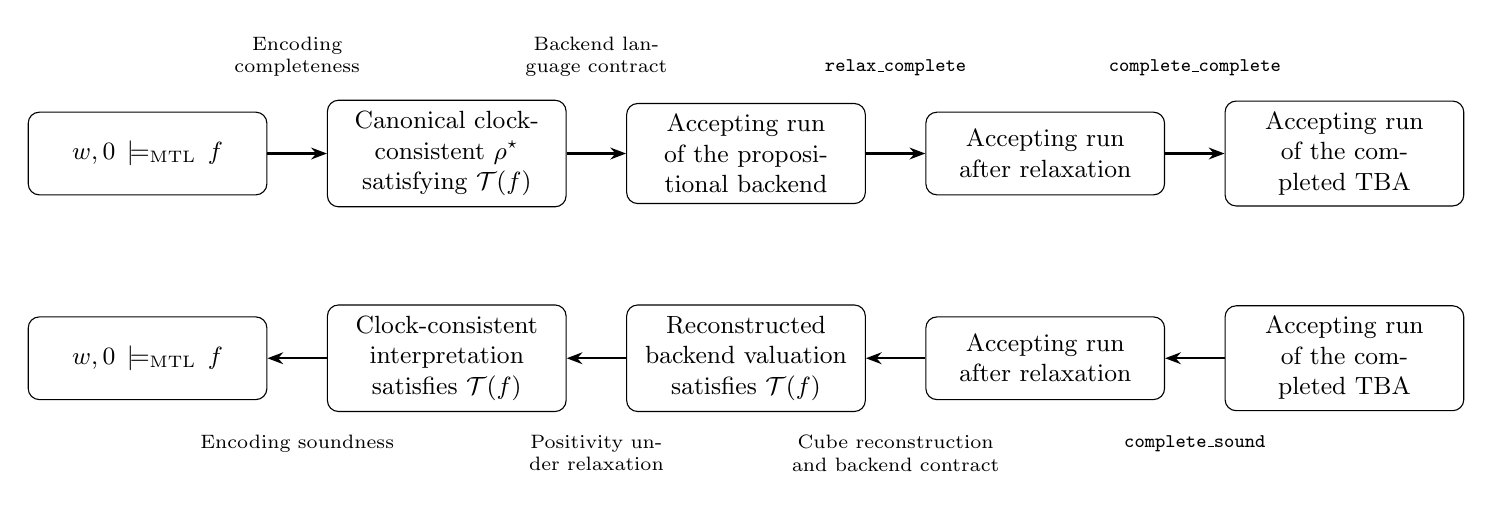
\begin{tikzpicture}[
  proofbox/.style={draw,rounded corners,align=center,text width=2.75cm,
    minimum height=1.05cm,font=\small,inner sep=4pt},
  flow/.style={-{Stealth[length=2mm]},thick},
  flowlabel/.style={font=\scriptsize,align=center,text width=2.65cm,fill=white}
]
\node[proofbox] (mtl) at (0,0) {$w,0\satM f$};
\node[proofbox] (enc) at (3.8,0) {Canonical clock-consistent
  $\rho^\star$ satisfying $\T(f)$};
\node[proofbox] (pb) at (7.6,0) {Accepting run of the
  propositional backend};
\node[proofbox] (relax) at (11.4,0) {Accepting run after
  relaxation};
\node[proofbox] (tba) at (15.2,0) {Accepting run of the
  completed TBA};
\draw[flow] (mtl.east) -- node[flowlabel,above=0.85cm] {Encoding
  completeness} (enc.west);
\draw[flow] (enc.east) -- node[flowlabel,above=0.85cm] {Backend language
  contract} (pb.west);
\draw[flow] (pb.east) -- node[flowlabel,above=0.85cm] {\texttt{relax\_complete}}
  (relax.west);
\draw[flow] (relax.east) -- node[flowlabel,above=0.85cm]
  {\texttt{complete\_complete}} (tba.west);

\node[proofbox] (mtls) at (0,-2.6) {$w,0\satM f$};
\node[proofbox] (encs) at (3.8,-2.6) {Clock-consistent
  interpretation satisfies $\T(f)$};
\node[proofbox] (pbs) at (7.6,-2.6) {Reconstructed backend
  valuation satisfies $\T(f)$};
\node[proofbox] (relaxs) at (11.4,-2.6) {Accepting run after
  relaxation};
\node[proofbox] (tbas) at (15.2,-2.6) {Accepting run of the
  completed TBA};
\draw[flow] (tbas.west) -- node[flowlabel,below=0.85cm]
  {\texttt{complete\_sound}} (relaxs.east);
\draw[flow] (relaxs.west) -- node[flowlabel,below=0.85cm]
  {Cube reconstruction and backend contract} (pbs.east);
\draw[flow] (pbs.west) -- node[flowlabel,below=0.85cm]
  {Positivity under relaxation} (encs.east);
\draw[flow] (encs.west) -- node[flowlabel,below=0.85cm]
  {Encoding soundness} (mtls.east);
\end{tikzpicture}}%
\caption{Proof outline for Theorem~\ref{thm:mtl-to-tba-correct}:
completeness (top) and soundness (bottom), each using the backend equivalence
contract.}
\label{fig:correctness-composition}
\end{figure*}

The convenience theorem \Rocqid{MTL_to_TBA_correct} chooses its backend
using the project axiom \Rocqid{LTL_TO_BUCHI_CORRECT}. It is not
assumption-free. The theorem displayed above instead takes backend
equivalence as an explicit argument. This distinction is visible in
\texttt{proof/ASSUMPTIONS.txt}; the concrete alarm example below proves a
contract for one Rocq backend record and does not rely on Spot being verified.

\subsection{Rocq result map and assurance boundary}
\label{subsec:rocq-result-map}
Table~\ref{tab:rocq-result-map} maps the article's results to their checked
declarations and assumptions. The primitive rows collect the four soundness
and four canonical-completeness families, each with its strict variant.
\begin{table*}[t]
\centering
\caption{Mathematical results and Rocq assurance boundary.}
\label{tab:rocq-result-map}
\begin{tabular}{@{}p{0.18\textwidth}p{0.32\textwidth}p{0.10\textwidth}p{0.26\textwidth}@{}}
\toprule
Mathematical result & Rocq declaration(s) & Source module & Key dependency\\
\midrule
Derived ordinary-operator semantics &
Eight strict/non-strict compatibility lemmas &
Core &
Well-formed real bounds and strictly increasing timed words\\
Canonical correctness at each path; one extension &
\Rocqid{canonical_encoding_all};
\Rocqid{EncodingCorrect_proved} &
Proof &
Standard Rocq real/classical and function-extensionality assumptions\\
Primitive soundness and canonical completeness &
\Rocqid{sound_UhatLe/Ge/Lt/Gt},
\Rocqid{sound_RhatLe/Ge/Lt/Gt};
corresponding \Rocqid{complete_*} lemmas &
Proof &
Soundness: any consistent resets; completeness: canonical policy\\
Relaxation and reset completion &
\Rocqid{relax_sound}, \Rocqid{relax_complete},
\Rocqid{complete_complete} &
Core &
Positive extended atoms; label side conditions\\
Conditional backend composition &
\Rocqid{MTL_to_TBA_correct_with} &
Proof &
Explicit all-propositional-words backend equivalence premise\\
Convenience backend theorem &
\Rocqid{MTL_to_TBA_correct} &
Proof &
Project axiom plus standard Rocq assumptions\\
Alarm-response instance &
\Rocqid{alarm_response_spot_backend_contract};
\Rocqid{alarm_response_spot_tba_correct} &
Alarm &
Contract proved for the Rocq record; Spot transcription is external\\
\bottomrule
\end{tabular}
\end{table*}

The source-module aliases in Table~\ref{tab:rocq-result-map} are:
\begin{description}
\item[Core.] \texttt{MTL\_to\_TBA\_Shared\_}\\
\texttt{Clock\_Derived\_Strict\_Direct\_Core.v}
\item[Proof.] \texttt{EncodingCorrect\_Shared\_}\\
\texttt{Clock\_Derived\_Strict\_Direct\_Proof.v}
\item[Alarm.] \texttt{OverlappingResponse\_Example.v}
\end{description}

The audit lists standard library dependencies for classical real comparison
decisions, excluded middle, functional extensionality, and descriptions.
These are distinct from the project-specific backend axiom. The theorem
\Rocqid{MTL_to_TBA_correct_with} has no
\Rocqid{LTL_TO_BUCHI_CORRECT} dependency; its backend premise
is explicit. The convenience theorem does use that axiom. The alarm-response
backend contract itself is proved for the Rocq \texttt{PBuchi} record under
the standard/classical assumptions in the audit.

The formal domain remains deliberately bounded: well-formed core formulas;
real-valued mathematical parameters (not executable encodings of arbitrary
reals); strictly increasing divergent timestamps; event-guarded automata
without location invariants; and existential nonnegative initial clock
values. The zero lower-bound and zero strict upper-bound reductions described
in Section~\ref{sec:mtl} are preprocessing, not mechanized results. Parsing,
a concrete LTL backend implementation, Spot execution, graph import,
automaton printing, and adaptation to zero-initialized clocks remain outside
the theorem. No runtime, state-size, or performance result is claimed.

The occurrence-indexed induction, residual invariants, and separate
relaxation/reset-completion obligations expose the proof dependencies behind
the language-preservation result. The development is supplied as inspectable
Rocq source; the successful source replay procedure and its limits are
documented with the artifact.
\subsection{Alarm-response proof instance}
\label{sec:alarm-example}
Consider $f_{\mathit{alarm}}=\mathsf{G}(\mathit{alarm}\Rightarrow
\Diamond_{\le 3}\mathit{handled})$, meaning every alarm must be handled within
three time units. In
\Rocqid{proof/OverlappingResponse_Example.v}, the formula is
\texttt{MR MFalse (MOr (MNotAtom ALARM) (MUle 3 MTrue (MAtom HANDLED)))},
where \texttt{ALARM} and \texttt{HANDLED} are actions 1 and 2. Rocq checks
that it is well formed and has one primitive timed subformula,
$\widehat{\mathsf{U}}_{\le 3}\,\top\,\mathit{handled}$, whose obligations
share clock $x$. Abbreviate $\mathsf{LAct}(\mathit{alarm})$ by $A$,
$\mathsf{LNAct}(\mathit{alarm})$ by $N$,
$\mathsf{LAct}(\mathit{handled})$ by $H$, $x\le3$ by $C$, and
$\mathsf{LUnch}(x)$ by $U$. Spot receives the exact clocked-LTL formula
\[
\mathsf{G}\bigl(N\lor H\lor \Next((C\land U)\Until(C\land H))\bigr).
\]
Spot 2.16's input and output are saved in
\Rocqid{examples/spot/alarm_response_backend.ltl} and
\Rocqid{examples/spot/alarm_response_backend.dot}~\cite{[spot]}. The generated graph has
initial state 0, accepting set $\{0,1\}$, and these transitions:
\[
\begin{array}{c|c|l}
\text{source}&\text{target}&\text{label}\\ \hline
0&0&H\lor N\\
0&1&\neg H\land\neg N\\
1&0&C\land H\\
1&2&C\land\neg H\land U\\
2&0&C\land H\\
2&2&C\land\neg H\land U
\end{array}
\]
The graph is manually transcribed as
\Rocqid{alarm_response_spot_backend}; Rocq splits the disjunctive
self-loop into two cubes. Lemma
\Rocqid{alarm_response_T_eq} matches its input to the Rocq translation;
\Rocqid{alarm_response_spot_backend_contract} proves that the transcribed
automaton has exactly that LTL language on all propositional words. This
discharges the backend premise for this instance. The regeneration script
requires \texttt{ltl2tgba --version} to report Spot 2.16.

The resulting concrete TBA is \Rocqid{alarm_response_spot_tba}. It has initial
location $0$, accepting locations $\{0,1\}$, and clock $x$. Table~\ref{tab:alarm-tba}
lists the reset-completed transitions in the Rocq record. Guards are checked
before resets, and $\top$ denotes no clock guard.
\begin{table}[t]
\centering
\caption{Timed transitions of the alarm-response Rocq record after
relaxation and reset completion. The Graphviz DOT graph-to-record correspondence remains
outside the Rocq proof.}
\label{tab:alarm-tba}
\begin{tabular}{@{}p{0.07\columnwidth}p{0.07\columnwidth}p{0.34\columnwidth}p{0.15\columnwidth}p{0.13\columnwidth}@{}}
\toprule
From & To & Event & Guard & Reset\\
\midrule
0 & 0 & $H$ & $\top$ & $\{x\}$\\
0 & 0 & $\neg A$ & $\top$ & $\{x\}$\\
0 & 1 & $A\land\neg H$ & $\top$ & $\{x\}$\\
1 & 0 & $H$ & $x\le3$ & $\{x\}$\\
1 & 2 & $\neg H$ & $x\le3$ & $\varnothing$\\
2 & 0 & $H$ & $x\le3$ & $\{x\}$\\
2 & 2 & $\neg H$ & $x\le3$ & $\varnothing$\\
\bottomrule
\end{tabular}
\end{table}
The theorem \Rocqid{alarm_response_spot_tba_correct} instantiates
Theorem~\ref{thm:mtl-to-tba-correct} and proves that this record accepts
exactly the timed words satisfying $f_{\mathit{alarm}}$. The verified object
is the Rocq record and its contract; neither Spot nor the saved DOT-to-record
transcription is verified.

Two trace instances make the universal theorem concrete. The accepted word
has alarms at times $0$ and $\tfrac32$, a handled event at time $3$, and only
neutral actions at subsequent timestamps, which advance by $\tfrac32$.
Rocq proves \Rocqid{alarm_overlap_trace_satisfies} and derives
\Rocqid{alarm_overlap_trace_accepted_by_spot_tba}. Both alarms use the same
clock $x$. On the canonical extension, the residual checks at indices 0 and 1
are respectively
\[
  0+(3-0)=3\le3,
  \qquad
  \tfrac32+(3-\tfrac32)=3\le3.
\]
Thus the clock is preserved at the second alarm: its existing value still
leaves exactly enough time for the shared handler at time 3. The accepted-trace
corollary follows from the checked MTL satisfaction proof and
\Rocqid{alarm_response_spot_tba_correct}; it is not a separate graph search.

The rejected word has alarms at times $0$ and $2$, a handled event at time
$4$, and neutral actions thereafter at intervals of 2. The first request has
no handler by time 3. Rocq proves
\Rocqid{alarm_response_trace_violates} and derives
\Rocqid{alarm_response_trace_rejected_by_spot_tba}. These are fixed trace
instances of the semantic result, not performance experiments or validation
of Spot's implementation.

The repository also provides a Python consistency check between the saved
graph and Rocq record (up to state renaming, including guards), with mutation
self-tests for a changed guard and accepting set. It is an executable audit of
the transcription, not a verified importer or a proof of Spot's semantics.
The separate finite reset-policy scenario is illustrative.

\section{Artifact and Reproducibility}
\label{sec:artifact}
The accompanying artifact contains the Rocq source modules, checked-in
assumptions audit, Spot inputs and saved graphs, assurance scripts, and the
Access manuscript source. From the \texttt{ieee\_access} directory, run
\texttt{reproduce-ieee-access.ps1}. This single entry point requires Rocq
9.0.1, Python 3, \texttt{pdflatex}, and BibTeX. It copies the proof sources to
a fresh temporary directory, compiles the core, correctness development, and
alarm example, independently checks the resulting proof objects, regenerates
the assumptions report and compares it with the checked-in audit without
overwriting that audit, runs the two Python assurance scripts, and builds the
PDF. A failing stage stops the script and reports its exit failure.

The main checked claims have direct source declarations:
\Rocqid{EncodingCorrect\_proved} and
\Rocqid{canonical\_encoding\_all} establish the formula-to-clocked-LTL
equivalence; \Rocqid{MTL\_to\_TBA\_correct\_with} composes this result with
the explicit all-propositional-words backend contract;
\Rocqid{alarm\_response\_spot\_tba\_correct} is the concrete alarm
instance. The primitive theorem families, relaxation lemmas, reset-completion
lemmas, and their assumptions are mapped in
Table~\ref{tab:rocq-result-map} and the checked-in \texttt{proof/ASSUMPTIONS.txt}.
The helper scripts compare the saved graph and Rocq record, or run the
illustrative finite reset-policy scenario; the Rocq development carries the
formal correctness claims.

Optional Spot 2.16 graph regeneration uses
\path{examples/spot/regenerate.sh}. It is not part of the reproduction
command, and no regeneration result is claimed.

The source and matching Portable Document Format (PDF) are included in the
local artifact candidate prepared for submission as supplementary material.
The public repository \url{github.com/efares1/}\allowbreak%
\url{coq-verified-mtl-to-tba} is mutable and does not yet identify this
revised Access snapshot. The candidate
\path{ieee-access-paper1-submission-v3} includes a manifest of Secure Hash
Algorithm 256 (SHA-256) digests for its packaged files; no public tag, release,
Digital Object Identifier (DOI), or third-party replay is claimed. Rebuilds
need not produce byte-identical PDF files; the packaged PDF is the designated
build.

\section{Related Work}
\label{sec:related}
\begin{table*}[!t]
\centering
\caption{Representative mathematical results and mechanization evidence for
timed-logic-to-automata constructions. The rows have different logics,
semantics, targets, and proof scopes; they are not a performance comparison.}
\label{tab:prior-construction-comparison}
\begin{tabular}{@{}p{0.12\textwidth}p{0.20\textwidth}p{0.34\textwidth}p{0.23\textwidth}@{}}
\toprule
Work & Semantic scope & Existing correctness and construction & Mechanization and implementation evidence\\
\midrule
Bulychev~\cite{[BDLG14]} & Pointwise non-Zeno infinite words; integer bounds, all four comparisons, nondecreasing timestamps. & Theorems 1--2 prove exact automaton languages for safety/co-safety. The construction already uses timed-subformula clocks, obligations, and reset/unchanged markers. & Mathematical proofs and controller-synthesis tooling for the stated fragments.\\
Li et al.~\cite{li_spin7} & Full MTL$_{0,\infty}$; pointwise non-Zeno words, integer bounds, all four comparisons, nondecreasing timestamps, zero initial clocks. & Establishes exact language equality for the timed-B\"uchi construction and language preservation under best-choice resets. & CASAAL implements the workflow and deterministic approximations~\cite{casaal_tool}; the proof is mathematical.\\
Xu and Miao~\cite{xu08} & MITL formulas mapped to fair timed automata; exact semantic relation to this paper's pointwise event-word model is not compared. & The article describes a syntax/semantics-based construction by formula type. & The publisher abstract reports PVS implementation details; detailed proof coverage is not assessed in this comparison.\\
This paper & Well-formed Rocq formulas with real bounds, strictly increasing timestamps, existential nonnegative initial clocks. & \Rocqid{EncodingCorrect_proved} proves clocked-LTL equivalence for all eight primitive cases; TBA composition is conditional on backend equivalence. & Rocq-checked proof and one proved contract for a manual Spot transcription; no executable MTL compiler or performance comparison.\\
\bottomrule
\end{tabular}
\end{table*}

Pointwise MTL has extensive decidability and expressiveness results
\cite{[RK90],[RTH96],MTLsem,ouaknine_worrell_lics05,
bouyer_chevalier_markey_fsttcs05}. Unrestricted dense-time MTL has no general
effective translation to finite ordinary timed automata; bounded-variability
and alternating-automaton results have different scopes
\cite{nickovic_piterman_formats10,[BM14]}. MTL$_{0,\infty}$ retains common
response and separation properties~\cite{[RTH96],[BDLG14]}. Our hatted
operators make the timing reference explicit in the logic and proof.

\runinhead{Translations of timed logics.}
Li et al. establish the full-fragment mathematical language-equivalence
result. Our overlapping-activation proof checks completeness for the present
formal model; we do not infer that prior constructions lacked such handling.

Xu and Miao describe a PVS-based transformation from MITL formulas to fair
timed automata, including construction principles and implementation
details~\cite{xu08}. This is an earlier proof-assistant-based timed-logic
translation; our scope-specific comparison concerns the pointwise
MTL$_{0,\infty}$ construction formalized here.

MITL translations use temporal testers, automata networks, or one-clock
alternating automata~\cite{maler_mitl_to_ta,
ferrere2019_realtimelogic_to_ta,[BM14]}; MightyL and MITL2Timed provide
UPPAAL-oriented tools for that distinct logic
\cite{mightyl_paper17,mitl2timed_github}. Obligation-merging techniques are
related, while our one-sided residual predicates support the checked
completeness proof.

\runinhead{Clocked temporal logic and subformula clocks.}
The clocked linear temporal logic extension CLTLoc adds clock comparisons and reset predicates and has been used to
encode metric logics~\cite{bersani_cltloc}. Our similar propositional
vocabulary is an automaton-synthesis intermediate: the backend treats clock
tests and reset markers as propositions. Positivity gives upward closure, and
reset completion restores timed meaning; hence the explicit relaxation proof.

Event-clock logics associate clocks with subformulas to measure time since or
until events~\cite{afh_eventclock_tcs99,
raskin_schobbens_jalc99,nickovic_piterman_formats10}. Formula-indexed clocks
are established; our proof checks that one clock per distinct timed formula
preserves language across repeated activations and all strict and non-strict
cases (Section~\ref{subsec:occurrence-induction}).

\runinhead{Recent automata-based real-time verification.}
Recent neighboring work addresses different settings: an improved one-clock
alternating MTL automaton for finite timed words with clock deactivation and
zone analysis~\cite{bouyer_srivathsan_vishwanath_fossacs25}; and TEMPORA's
pointwise MITL model checking with past and future modalities
~\cite{akshay_et_al_tempora26}. These do not
translate our MTL$_{0,\infty}$ fragment to infinite-word TBAs.
Ho et al.'s MightyPPL translates pointwise MITL with past and Pnueli
modalities over finite and infinite timed words; it gives mathematical
construction results and proof sketches alongside a complete implementation
whose testers sequentialize overlapping obligations
\cite{mightyppl_tacas26}. The September 2026 QEST+FORMATS preprint describes
an implementation for existentially punctual metric temporal logic with past
and Pnueli modalities (MTLPPL)~\cite{mightyppl_qest_arxiv26}. Its term
\emph{one-sided MTL} denotes the subfragment without past or Pnueli, whereas
here it describes interval shapes $[0,d]$ and $[d,\infty)$. Any syntactic
containment comparison is limited to conventional source formulas after
zero-bound reduction and with integer bounds; it excludes hatted abstract syntax tree (AST)
constructors. The QEST fragment also permits punctual and non-one-sided
intervals in its stated positions. Its punctual-response example does not
imply support for unrestricted punctual MTL; differing bounds and timed-word
conventions preclude a shared-input semantic comparison.

These tools address different fragments or output models; this paper neither
re-verifies them nor makes a shared-input, coverage, clock-count, or
performance comparison. The Rocq development is not integrated with CASAAL,
MightyPPL, or another checker.

\runinhead{Mechanized translations and trusted backends.}
Proof-assistant work already verifies LTL-to-B\"uchi constructions and model
checkers~\cite{schimpf_tphols09,cava_cav13,ltl_to_gba_afp,
seidl_sickert_afp19}. Wang et al. verify an MLTL-to-regular-expression
transformation in Isabelle/HOL, export executable code, and compare it with
existing implementations~\cite{wang_mltl_tacas25}. Chattopadhyay and
Mamouras formalize in Coq a compositional construction of online monitors for
past-time MTL over a discrete temporal domain, using quantitative semantics
and Moore machines; they also extract OCaml monitors. This is a distinct
monitoring target and semantic setting from the infinite-word TBA construction
studied here~\cite{chattopadhyay_mamouras_rv20}. For metric logics, Roohi
and Viswanathan use PVS to correct an unsound release semantics in prior MITL
decision procedures and prove supporting results for an adapted
timed-automata construction under continuous-time signal semantics
~\cite{roohi_viswanathan_vmcai18}. Xu and Miao's PVS-based construction is
described above. Together, these works establish substantial proof-assistant
precedents for related metric logics, monitors, and automata; this paper adds a
Rocq-checked correctness development for the specified pointwise infinite-word
TBA construction.

\runinhead{Event-B refinement patterns.}
Our work on Event-B patterns addresses their generation and refinement,
including domain-specific language (DSL)-based pattern generation~\cite{fares_abz23}, patterns using
weakest-precondition calculus~\cite{fares_facs24}, and a forthcoming 2027
article on pattern-based development using predicate transformers~\cite{fares_scp27}. These works
provide the Event-B pattern-generation context for our broader objective:
given an MTL property, use its TBA translation as the input to a downstream
Event-B pattern-generation step. The present paper establishes the MTL-to-TBA
stage only. It gives no TBA-to-Event-B transformation or correctness result
for generated Event-B patterns.

\section{Conclusion}
This paper provides a Rocq-checked soundness-and-completeness development for
the specified pointwise MTL$_{0,\infty}$-to-TBA construction. Its proof covers
all eight strict and non-strict primitive cases, soundness for arbitrary
clock-consistent reset traces, and completeness using one canonical trace
across repeated activations of formula-keyed clocks. The occurrence-indexed
induction connects each syntactic occurrence to its translation while
preserving the identity of a shared clock. This supplies a checked account of
the obligations that a mathematical argument must discharge when several
timed requirements overlap.

Rocq also checks relaxation and reset completion and composes them with an
explicit propositional backend language-equivalence contract. The resulting
theorem makes its backend dependency inspectable instead of hiding it in an
assurance claim. This work builds on the mathematical language-preservation
results of Li et al. and adjacent proof-assistant work, while contributing a
machine-checked derivation for the formal construction and semantic model
defined here~\cite{li_spin7,xu08,roohi_viswanathan_vmcai18}.

For the alarm-response instance, the backend contract is proved for a manual
Rocq transcription of a Spot graph. Rocq proves both acceptance of the
overlapping-request trace, whose response satisfies the concurrent
obligations, and rejection of a fixed violating trace. These examples make
the theorem concrete; the external graph-to-record path remains outside its
proof. The theorem applies to the stated pointwise semantics and composes
through an explicit backend contract; Spot's graph generation/import and
zero-bound preprocessing remain outside the checked boundary. Future work
can extend the mechanization to these components and connect the semantic
theorem to a verified executable backend.


\bibliographystyle{IEEEtran}
\bibliography{references}
\begin{IEEEbiographynophoto}{Elie Fares}
Elie Fares is with the Higher Colleges of Technology, Sharjah, United Arab
Emirates. His research interests include formal methods, timed systems, and
mechanized verification.
\end{IEEEbiographynophoto}

\begin{IEEEbiographynophoto}{Jean-Paul Bodeveix}
Jean-Paul Bodeveix is with IRIT, Universit\'e de Toulouse, France. His
research interests include formal methods, proof assistants, and model
checking.
\end{IEEEbiographynophoto}

\begin{IEEEbiographynophoto}{Hussain Al-Aqrabi}
Hussain Al-Aqrabi is with the Higher Colleges of Technology, Sharjah, United
Arab Emirates. His research interests include cybersecurity and cloud
security.
\end{IEEEbiographynophoto}

\begin{IEEEbiographynophoto}{Azar Salami}
Azar Salami is with the Higher Colleges of Technology, Sharjah, United Arab
Emirates. He received the Ph.D. degree in mathematics from Universit\'e Laval,
Canada. His research interests include mathematical modeling and formal
methods.\EOD
\end{IEEEbiographynophoto}
\end{document}
